\chapter{不变子空间}

事实上,为了研究上一讲前言中提到的线性变换、矩阵和多项式之间的关系,我们需要一个重要的媒介,即不变子空间. 相信读者这一点在接下来的章节中会逐渐体会到这一概念的桥梁作用.

\section{不变子空间的定义}

回顾我们接下来讨论的目标,即找到一组基使得线性变换在这组基下的表示更简单. 设$\sigma\in\mathcal{L}(V)$,如果$V$有直和分解
\begin{equation}\label{eq:18:直和分解}
    V=U_1\oplus U_2\oplus\cdots\oplus U_m,
\end{equation}
其中每个$U_i$都是$V$的真子空间,那么我们对于$\sigma$的研究可以分别在各个$U_i$上进行. 这其中的基本原理在于直觉告诉我们(并且实际上通常而言)更低维的空间处理起来应当更为简单,事实上我们后面的很多工作都是在找这样的分解.

为了在低维空间上进行研究,我们需要引入一个新的概念,即$\sigma$在$U_i$下的限制映射$\sigma\vert_{U_i}$. 我们给出标准的定义如下:
\begin{definition} \index{xianxingyingshe!xianzhi@限制 (restriction map)}
    设$V$是数域$\mathbf{F}$上的线性空间,$\sigma\in\mathcal{L}(V)$,我们在$V$的子空间$U$上定义映射$\sigma\vert_U$如下:
    \[\sigma\vert_U:U\to V,\enspace\sigma\vert_U(\alpha)=\sigma(\alpha),\enspace\forall \alpha\in U,\]
    则称$\sigma\vert_U$是$\sigma$在$U$上的\term{限制映射}.
\end{definition}

``限制''一词十分形象(如下图所示),因为限制映射就是将原映射的定义域限制在更小的范围内,但原定义域上的映射值保持不变.
\begin{figure}[H]
    \centering
    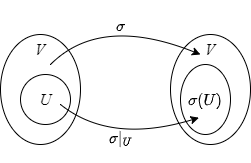
\includegraphics[scale=0.7]{figs/18-1.png}
\end{figure}

但是我们需要注意,\autoref{eq:18:直和分解}这一分解应当满足一个基本的条件,就是$\sigma$应当把每个$U_i$仍然映射到$U_i$本身,否则我们在讨论$\sigma\vert_{U_i}$的时候它不是一个线性变换,这与我们讨论的主题不一致,即我们希望限制映射$\sigma\vert_{U_i}$是一个线性变换(是$\mathcal{L}(U_i)$中的元素),我们称之为\term{限制线性变换}\index{xianxingbianhuan!xianzhi@限制线性变换 (restriction operator)}.

事实上,满足$\sigma\vert_{U_i}\in\mathcal{L}(U_i)$的子空间$U_i$非常重要,我们需要给予它一个定义:
\begin{definition}
    设$\sigma\in \mathcal{L}(V)$,若$V$的子空间$U$满足$\forall \alpha\in U,\enspace \sigma(\alpha)\in U$,则称$U$是$\sigma$的\term{不变子空间}\index{xianxingkongjian!zi!bubian@不变子空间 (invariant subspace)},或称$U$在$\sigma$下不变,简称为$\sigma$-子空间.
\end{definition}
即不变子空间中的每一个向量经过映射后仍在这一空间中,因此这里的``不变''的含义也是非常直观的. 根据定义我们可以验证或者求解一些很简单的不变子空间. 教材例5.3给出了四个常见的不变子空间的例子,分别是两个平凡子空间和映射的像与核,验证非常简单,此处不赘述. 教材8.20还给出了$p$为多项式时,$\ker p(\sigma)$和$\im p(\sigma)$也为$\sigma$的不变子空间. 我们这里也简要书写一下,供读者熟悉如何利用定义验证不变子空间:
\begin{example}
    若$\sigma\in\mathcal{L}(V)$且$p\in\mathbf{F}[x]$为多项式,则$\ker p(\sigma)$和$\im p(\sigma)$在$\sigma$下不变.
\end{example}

\begin{proof}
    我们只需验证$\ker p(\sigma)$和$\im p(\sigma)$中的元素经过$\sigma$映射后仍在这一空间中即可.
    \begin{enumerate}
        \item $\forall \alpha\in \ker p(\sigma),\enspace p(\sigma)\alpha=0$,因此
        \[(p(\sigma))(\sigma(\alpha))=\sigma(p(\sigma)\alpha)=\sigma(0)=0,\]
        即$\sigma(\alpha)\in \ker p(\sigma)$,因此$\ker p(\sigma)$在$\sigma$下不变;

        \item $\forall \alpha\in \im p(\sigma),\enspace \exists \beta\in V,\enspace \alpha=p(\sigma)\beta$,因此
        \[\sigma(\alpha)=\sigma(p(\sigma)\beta)=p(\sigma)(\sigma(\beta))\in \im p(\sigma),\]
        即$\im p(\sigma)$在$\sigma$下不变.
    \end{enumerate}
    事实上,对于$\ker p(\sigma)$,我们有
    \[ p(\sigma)(\alpha)=p(\sigma)\alpha=p(\sigma(\alpha))=p(0)=0,\]
    因此$\sigma(\alpha)\in \ker p(\sigma)$,即$\ker p(\sigma)$在$\sigma$下不变. 对于$\im p(\sigma)$,我们有
    \[\forall \alpha\in \im p(\sigma),\enspace \exists \beta\in V,\enspace \alpha=p(\sigma)\beta,\]
    因此
    \[\sigma(\alpha)=\sigma(p(\sigma)\beta)=p(\sigma)\sigma(\beta)\in \im p(\sigma),\]
    即$\im p(\sigma)$在$\sigma$下不变.
\end{proof}

有时我们可能会遇到更为复杂的情形,如下面的例子:
\begin{example} \label{ex:18:不变子空间}
    设$\mathbf{F}$为一数域,线性变换$\sigma\in\mathcal{L}(\mathbf{F}^2)$定义为
    \[\sigma(a,b)=(a,b)\begin{pmatrix}
            1 & -1 \\ 2 & 2
        \end{pmatrix}\]
    证明:
    \begin{enumerate}
        \item 当$\mathbf{F}=\mathbf{R}$时,$\mathbf{R}^2$无$\sigma$的非零真不变子空间;

        \item 当$\mathbf{F}=\mathbf{C}$时,$\mathbf{C}^2$有$\sigma$的非零真不变子空间.
    \end{enumerate}
\end{example}

\begin{proof}
    事实上,由于$\sigma$定义在二维空间$\mathbf{F}^2$上,因此``非零真不变子空间''只能是一维子空间. 设该不变子空间$U=\spa(\alpha)(\alpha\neq 0)$,并进一步设$\alpha=(a,b)$. 我们知道,一维线性空间中所有元素都是成比例的(可以理解为一条直线,或者一维空间是由一个向量线性扩张而来,扩张过程中的线性组合一定保证后面生成的所有向量都互相成比例). 我们假设比例值为$\lambda$,即
    \[\sigma(a,b)=(a,b)\begin{pmatrix}
            1 & -1 \\ 2 & 2
        \end{pmatrix}=\lambda(a,b)=(\lambda a,\lambda b),\]
    将矩阵乘法展开,我们有
    \[(a+2b,-a+2b)=(\lambda a,\lambda b).\]
    由于$\alpha=(a,b)\neq 0$,因此$\lambda\neq 0$,基于此解方程得到$\lambda^2-3\lambda+4=0$.这一方程在实数域范围内无解,复数域内有两个共轭的解,因此,我们有
    \begin{enumerate}
        \item 当$\mathbf{F}=\mathbf{R}$时,$\mathbf{R}^2$无$\sigma$的非零真不变子空间;

        \item 当$\mathbf{F}=\mathbf{C}$时,$\mathbf{C}^2$有$\sigma$的非零真不变子空间.
    \end{enumerate}
\end{proof}

除此之外,还有一些更为困难的问题我们将在讨论若当标准形之后进行讨论.

最后我们再基于不变子空间讨论一个商线性变换的概念. 事实上,如果$U$是$\sigma$的不变子空间,那么$\sigma$还可以诱导出商空间$V/U$上的线性变换. 我们严格定义如下:
\begin{definition}
    设$\sigma\in \mathcal{L}(V)$,$U$是$\sigma$的不变子空间,定义映射$\sigma/U:V/U\to V/U$如下:
    \[(\sigma/U)(v+U)=\sigma(v)+U,\enspace\forall v\in V,\]
    则称$\sigma/U$是$\sigma$在$U$上的\term{商线性变换}\index{xianxingbianhuan@shang!商线性变换 (quotient operator)}.
\end{definition}

定义映射后,我们自然的想法就失确认这一定义是不是合理的. 首先这一定义的线性性容易验证,我们只需要用到商空间中定义的运算性质即可:
\begin{itemize}
    \item 齐次性:$(\sigma/U)(\lambda(v+U))=(\sigma/U)(\lambda v+U)=\sigma(\lambda v)+U=\lambda\sigma(v)+U=\lambda(\sigma/U)(v+U)$;

    \item 加性:$(\sigma/U)((v_1+U)+(v_2+U))=(\sigma/U)(v_1+v_2+U)=\sigma(v_1+v_2)+U=\sigma(v_1)+\sigma(v_2)+U=(\sigma/U)(v_1+U)+(\sigma/U)(v_2+U)$.
\end{itemize}

除了线性的要求外,还有一个很重要的合理性来源于\autoref{ex:8:良定义} 中提到的良定义(well-defined)的概念. 因为这里又一次将线性变换定义在了等价类上,因此我们需要特别关注这一定义的良定义性. 事实上,回顾\autoref{ex:8:良定义},对于一个映射,其合理性在于原像集合中的一个元素只能映射到像集中的唯一一个值(否则不符合映射的定义). 商线性变换的出发空间元素是等价类,因此如果出现$v+U=w+U$但$\sigma(v)+U\neq \sigma(w)+U$的情况,这一定义描述的就不是映射(因为映射要求一个自变量只能映到一个值上),因此不是良定义. 但我们可以验证这一映射是良定义的:

\begin{proof}
    设$v+U=w+U$,即$v-w\in U$,由于$U$在$\sigma$下不变,则$\sigma(v-w)\in U$,即$\sigma(v)-\sigma(w)\in U$,因此$\sigma(v)+U=\sigma(w)+U$,即$\sigma/U$是良定义的.
\end{proof}

这一定义可能具有一定的抽象性,因此我们用更抽象的例子来加深理解:
\begin{example}
    设$\sigma\in \mathcal{L}(V,W)$,定义$\widetilde{\sigma}:(V/(\ker \sigma))\to W$如下:
    \[\widetilde{\sigma}(v+\ker\sigma)=\sigma(v).\]
    \begin{enumerate}
        \item $\widetilde{\sigma}$是良定义的,且是$(V/(\ker \sigma))$到$W$上的线性映射;

        \item $\widetilde{\sigma}$是单射;

        \item $\im \widetilde{\sigma}=\im \sigma$;

        \item $V/(\ker \sigma)$同构于$\im \sigma$.
    \end{enumerate}
\end{example}

\begin{proof}

\end{proof}

\section{特征值与特征向量}

事实上,在\autoref{ex:18:不变子空间} 中,我们求解了一维不变子空间. 根据一维空间中向量都成比例的性质,设$U$是$\sigma\in\mathcal{L}(V)$的一维不变子空间,我们有
\[\exists\lambda\in\mathbf{F},\enspace\sigma(\alpha)=\lambda\alpha,\enspace\forall \alpha\in U,\]
即任意向量作用线性变换后的结果与原向量成比例. 这一性质将引入接下来的特征值与特征向量的概念,事实上它们对于获得简单矩阵的目标而言非常重要,因此我们需要特别研究一维不变子空间.

在接下来的讨论中,我们很多定义都会有相应的矩阵和映射版本. 回顾在\autoref{thm:11:线性映射对向量坐标的影响} 中的讨论,我们提到了矩阵$A$和线性映射$\sigma(\alpha)=A\alpha$的统一性,提到我们未来将不区分矩阵和线性变换,这一点在本节过后将有更深刻的体会.

\subsection{特征值与特征向量的定义与求解}

首先介绍线性变换和矩阵的特征值与特征向量的概念:
\begin{definition}
    设$\sigma$是线性空间$V(\mathbf{F})$上的一个线性变换,如果存在数$\lambda\in\mathbf{F}$和非零向量$\xi\in V$使得$\sigma(\xi)=\lambda\xi$,则称数$\lambda$为$\sigma$的一个\term{特征值}\index{tezhengzhi@特征值 (eigenvalue)},并称非零向量$\xi$为$\sigma$属于其特征值$\lambda$的\term{特征向量}\index{tezhengxiangliang@特征向量 (eigenvector)}.
\end{definition}
必须注意特征向量为非零向量,否则零向量$\xi=\vec{0}$对任意$\lambda$都满足上面定义,从而失去``特征''的含义. 但是特征值可以为0,此时$\sigma(\xi)=\vec{0}$,即全体特征向量的集合就是线性变换的核空间.

对于某一个$\lambda\in\mathbf{F}$,我们将所有满足$\sigma(\xi)=\lambda\xi$的向量构成的集合记为$V_\lambda=\{\xi \mid \sigma(\xi)=\lambda\xi,\enspace\xi\in V\}$,称为$\sigma$关于其特征值$\lambda$的\term{特征子空间}\index{tezhengzikongjian@特征子空间 (eigenspace)}. 显然,这一集合是由零向量和全体$\lambda$对应的特征向量构成的. 我们可以验证$V_\lambda$的确是$V$的``子空间'':
\begin{example}
    证明:$V_\lambda$是$V$的子空间.
\end{example}

\begin{proof}
    回顾证明子空间的两个要求:非空和运算封闭性. 首先$V_\lambda$非空,因为$\vec{0}\in V_\lambda$,即$\sigma(\vec{0})=\lambda\vec{0}$,因此$\vec{0}\in V_\lambda$,故$V_\lambda$非空.

    其次,对于任意$\xi_1,\xi_2\in V_\lambda$,$k_1,k_2\in\mathbf{F}$,我们有
    \[\sigma(k_1\xi_1+k_2\xi_2)=k_1\sigma(\xi_1)+k_2\sigma(\xi_2)=k_1\lambda\xi_1+k_2\lambda\xi_2=\lambda(k_1\xi_1+k_2\xi_2),\]
    因此$k_1\xi_1+k_2\xi_2\in V_\lambda$,故满足线性运算封闭. 综上,$V_\lambda$是$V$的子空间.
\end{proof}

事实上,我们通过之后的例子会知道,$V_\lambda$的维数不一定是1,而至少是1. 那么我们之前引入特征值特征向量时所说的``一维不变子空间''是什么呢?事实上,我们可以取$V_\lambda$的任一组基$\alpha_1,\ldots,\alpha_n$,则其中任一向量进行扩张得到的子空间$U_i=\spa(\alpha_i)(i=1,\cdots,n)$就是一维不变子空间,因为$\forall u_i\in U_i,\enspace \sigma(u_i)=\lambda u_i\in U_i$,即$U_i$在$\sigma$下不变. 我们还需要注意,一维不变子空间的选取是不唯一的,因为$V_\lambda$的基的选取是不唯一的,因此$U_i$的选取也是不唯一的,实际上对于任意的$\alpha\in\V_{\lambda}$,$\spa(\alpha)$都是一维不变子空间.

上面是线性变换的特征值与特征向量的定义,事实上我们也有对应的矩阵的特征值与特征向量的定义:
\begin{definition}
    设矩阵$A\in \mathbf{M}_n(\mathbf{F})$,如果存在数$\lambda\in\mathbf{F}$和非零向量$X\in\mathbf{F}^n$使得$AX=\lambda X$,则称数$\lambda$为$A$的一个特征值,称非零向量$X$为$A$属于其特征值$\lambda$的特征向量.
\end{definition}

下面我们说明线性映射的特征值与特征向量和矩阵的特征值与特征向量之间的关系. 实际上,假设$A$是$\sigma$在基$\alpha_1,\ldots,\alpha_n$下的表示矩阵,且$\xi=(\alpha_1,\ldots,\alpha_n)X$,即$X$是$\xi$在基$\alpha_1,\ldots,\alpha_n$下的坐标,则我们有
\begin{align*}
    \sigma(\xi)=\lambda\xi & \iff \sigma((\alpha_1,\ldots,\alpha_n)X)=\lambda(\alpha_1,\ldots,\alpha_n)X        \\
                           & \iff (\sigma(\alpha_1,\ldots,\alpha_n))X=(\lambda\alpha_1,\ldots,\lambda\alpha_n)X \\
                           & \iff (\alpha_1,\ldots,\alpha_n)AX=(\alpha_1,\ldots,\alpha_n)(\lambda X)            \\
                           & \iff AX=\lambda X
\end{align*}
其中第一行与第二行间的等价关系用到了矩阵乘法一节中证明的性质$\sigma((\alpha_1,\ldots,\alpha_n)X)=(\sigma(\alpha_1,\ldots,\alpha_n))X$. 由上述讨论可知$\lambda$同时是线性变换和矩阵的特征值,与基的选取无关. 但矩阵的特征向量$X$是线性映射特征向量在基下的坐标,这与基的选取有关.

接下来我们讨论如何求解特征值与特征向量. 我们首先需要证明一个定理:
\begin{theorem}
    设$\sigma$是$V(\mathbf{F})$上的线性变换,$I$为恒等映射,则下述条件等价:
    \begin{enumerate}[label=(\arabic*)]
        \item \label{item:18:特征值定义:1}
              $\lambda\in\mathbf{F}$是$\sigma$的特征值;

        \item \label{item:18:特征值定义:2}
              $\sigma-\lambda I$不是单射;

        \item \label{item:18:特征值定义:3}
              $\sigma-\lambda I$不是满射;

        \item \label{item:18:特征值定义:4}
              $\sigma-\lambda I$不可逆.
    \end{enumerate}
\end{theorem}

\begin{proof}
    \begin{itemize}
        \item[\ref*{item:18:特征值定义:1}$\implies$\ref*{item:18:特征值定义:2}] $\lambda\in\mathbf{F}$是$\sigma$的特征值,说明$\exists v\in V$且$v\neq 0$使得$\sigma(v)=\lambda v$. 因此$(\sigma-\lambda I)(v)=0$,即$\sigma-\lambda I$核空间不只有零元,根据单射等价条件\autoref{thm:5:单射与核空间},不单成立;

        \item[\ref*{item:18:特征值定义:2}$\implies$\ref*{item:18:特征值定义:3}] 根据\autoref{thm:6:双射等价条件} 可知,$\sigma-\lambda I$不满当且仅当$\sigma-\lambda I$不单;

        \item[\ref*{item:18:特征值定义:3}$\implies$\ref*{item:18:特征值定义:4}] 根据\autoref*{thm:6:双射等价条件} 显然;

        \item[\ref*{item:18:特征值定义:4}$\implies$\ref*{item:18:特征值定义:1}] $\sigma-\lambda I$不可逆,根据\autoref*{thm:6:双射等价条件} 可知其不为单射,又根据单射等价条件\autoref*{thm:5:单射与核空间} 可知$(\sigma-\lambda I)(v)=0$有非零解,即$\sigma(v)=\lambda v$,其中$v\neq 0$,这与特征值定义一致.
    \end{itemize}
\end{proof}

由上述定理,$\lambda\in\mathbf{F}$是$\sigma$的特征值等价于$\sigma-\lambda I$不可逆,因此其在$V$的任意一组基$\alpha_1,\ldots,\alpha_n$下的矩阵$A-\lambda E$也不可逆(其中$A$为$\sigma$在这组基下的矩阵,$E$为单位矩阵),这又等价于$|A-\lambda E|=0$.

因此$\lambda\in\mathbf{F}$是$\sigma$的特征值等价于$|\lambda E-A|=0$,故我们可以通过$|\lambda E-A|=0$求解特征值,其中$A$为$\sigma$在某组基下的矩阵,$E$为单位矩阵对于特征向量的求解,求出$(\lambda E-A)X=0$的非零解就是特征向量在基$\alpha_1,\ldots,\alpha_n$下的坐标,如果是矩阵的特征向量,那么$X$就是解.

上述求解特征向量的方法需要我们求解$f(\lambda)=|\lambda E-A|$的根,事实上$f(\lambda)=|\lambda E-A|$是在之后的讨论中有核心地位的概念,我们称其为矩阵$A$的\term{特征多项式}{tezhengduoxiangshi@特征多项式 (characteristic polynomial)},其$k$重根称为$k$重特征值(称$k$为代数重数),该特征值对应的特征子空间维数称为该特征值的几何重数.

\begin{example}
    设$A=\begin{pmatrix}
            1 & -1 & 0 \\ 2 & 0 & 1 \\ 1 & a & 0
        \end{pmatrix}$,且存在非零向量$\alpha$使得$A\alpha=2\alpha$,求$a$.
\end{example}

\begin{solution}
    由题意知2是矩阵$A$的特征值,因此我们有
    \[|2E-A|=\begin{vmatrix}
            1 & 1 & 0 \\ -2 & 2 & -1 \\ -1 & -a & 2
        \end{vmatrix}=9-a=0,\]
    因此$a=9$.
\end{solution}

接下来,我们将特征多项式定义中的行列式展开得到以下定理:
\begin{theorem}\label{thm:18:特征多项式展开}
    对于$n$级矩阵$A=(a_{ij})$,记
    \[f(\lambda)=|\lambda E-A|=a_0\lambda^n+a_1\lambda^{n-1}+\cdots+a_{n-1}\lambda+a_n\]
    则$a_0=1$,$a_1=-\textup{tr}(A)$,$a_n=(-1)^n|A|$,且$a_k$等于所有$k$级主子式之和乘以$(-1)^k$.
\end{theorem}

\begin{proof}
    设$A=(a_{ij})$的列向量为$\alpha_1,\ldots,\alpha_n$,则
    \[f(\lambda)=|\lambda E-A|=\begin{vmatrix}
            \lambda e_1-\alpha_1 & \lambda e_2-\alpha_2 & \cdots & \lambda e_n-\alpha_n
        \end{vmatrix}.\]
    其中$e_1,\ldots,e_n$为$\mathbf{F}^n$的标准基,因此根据行列式的\autoref{def:13:公理化定义}的加性,$f(\lambda)$可以拆成$2^n$个行列式的和,它们是
    \begin{equation}\label{eq:18:特征多项式展开}
        (-\alpha_1,\cdots,-\alpha_{j_1-1},\lambda e_{j_1},-\alpha_{j_1+1},\cdots,-\alpha_{j_2-1},\lambda e_{j_2},-\alpha_{j_2+1},\cdots,-\lambda e_{j_{n-k}},\cdots,-\alpha_n),
    \end{equation}
    其中$1\leqslant j_1<j_2<\cdots<j_{n-k}\leqslant n,\enspace k=0,2,\ldots,n$.

    上式初看会显得非常复杂,但实际上利用行列式定义的加性去拆分就是每列有两种拆出来的选择,一种是选择$\lambda e_{j_i}$,另一种是选择$-\alpha_{j_i}$,这就是$2^n$种拆分方式的来由. 其中取出$k$列$-\alpha_{j_i}$,剩余$n-k$列选择$\lambda e_{j_i}$的就可以表示为上式的形式.

    利用\autoref{thm:14:Laplace定理}对\autoref{eq:18:特征多项式展开}第$j_1,\ldots,j_{n-k}$列展开,我们发现这$n-k$列元素组成的$n-k$阶子式只有一个不为0:
    \[\begin{vmatrix}
            \lambda & 0       & \cdots & 0       \\
            0       & \lambda & \cdots & 0       \\
            \vdots  & \vdots  & \ddots & \vdots  \\
            0       & 0       & \cdots & \lambda
        \end{vmatrix}=\lambda^{n-k},\]
    这个不等于0的$n-k$阶子式对应的代数余子式为
    \begin{align*}
        &(-1)^{(j_1+\cdots+j_{n-k})+(j_1+\cdots+j_{n-k})}(-A)\begin{pmatrix}
            j_1' & j_2' & \cdots & j_k' \\
            j_1' & j_2' & \cdots & j_k'
        \end{pmatrix} \\
        &= (-1)^kA\begin{pmatrix}
            j_1' & j_2' & \cdots & j_k' \\
            j_1' & j_2' & \cdots & j_k'
        \end{pmatrix}
    \end{align*}
    其中$j_1',\ldots,j_k'$为$1,\ldots,n$中除去$j_1,\ldots,j_{n-k}$的$k$个数按递增顺序排列的结果,这一点通过余子式的定义是显然的. 因此\autoref{eq:18:特征多项式展开}的值为
    \[(-1)^kA\begin{pmatrix}
            j_1' & j_2' & \cdots & j_k' \\
            j_1' & j_2' & \cdots & j_k'
        \end{pmatrix}\lambda^{n-k}.\]
    这实际上只是取$n-k$列$\lambda e_{j_i}$的一种情况,事实上对于所有可能的$j_1,\ldots,j_{n-k}$的取法,我们都可以得到类似的结果,因此$|\lambda E-A|$中$\lambda^{n-k}$的系数为
    \[(-1)^k\sum\limits_{1\leqslant j_1'<\cdots<j_k'\leqslant n}A\begin{pmatrix}
            j_1' & j_2' & \cdots & j_k' \\
            j_1' & j_2' & \cdots & j_k'
        \end{pmatrix}.\]
    即$a_k$等于所有$k$级主子式之和乘以$(-1)^k$,且代入$k=0,1,n$有$a_0=1$,$a_1=-\textup{tr}(A)$,$a_n=(-1)^n|A|$.
\end{proof}

这一定理的证明事实上无需掌握,这里给出证明是为了补全教材中的空缺. 这里我们主要掌握两个特例,即由韦达定理,我们有
\begin{enumerate}
    \item $\displaystyle\sum_{i=1}^{n}\lambda_i=\displaystyle\sum_{i=1}^{n}a_{ii}$;

    \item $\displaystyle\prod_{i=1}^{n}\lambda_i=|A|$.
\end{enumerate}
即特征值按重数求和为矩阵的迹(即矩阵对角线元素之和),特征值按重数求积为矩阵行列式. 这一结论在解决某些问题时有一定作用.

事实上,我们这里给出的特征多项式只是矩阵的特征多项式的定义,关于线性变换特征多项式的定义以及进一步讨论将在后续章节进行,我们也会说明两种特征多项式的定义是统一的.

\subsection{特征值的基本性质}

关于特征值,我们有如下基本性质:
\begin{enumerate}
    \item 设$\lambda$是线性空间$V(\mathbf{F})$上的线性变换$\sigma$的特征值,$\xi$是$\sigma$属于$\lambda$的特征向量,则
          \begin{enumerate}
              \item $k\lambda$是$k\sigma$的特征值,$\lambda^m$是$\sigma^m$的特征值,且$\xi$仍是相应特征向量;

              \item 若$f(x)=a_nx^n+a_{n-1}x^{n-1}+\cdots+a_1x+a_0$是$\mathbf{F}$上的多项式,则$f(\sigma)(\xi)=f(\lambda)\xi$;
          \end{enumerate}

    \item 设$\lambda$是$n$阶矩阵$A$的特征值,$A$可逆,则$\lambda^{-1}$是$A^{-1}$的特征值,$|A|\lambda^{-1}$是$A$的伴随矩阵$A^*$的特征值,且特征向量不变.
\end{enumerate}

\begin{proof}
\begin{enumerate}
    \item
    \begin{enumerate}
        \item 由于$\sigma(\xi)=\lambda\xi$,则$(k\sigma)(\xi)=k\lambda\xi$,即$k\lambda$是$k\sigma$的特征值,$\xi$仍是相应特征向量.

        而$\sigma^m(\xi)=\sigma^{m-1}(\sigma(\xi))=\sigma^{m-1}(\lambda\xi)=\lambda\sigma^{m-1}(\xi)=\cdots=\lambda^m\xi$,即$\lambda^m$是$\sigma^m$的特征值,$\xi$仍是相应特征向量.

        \item 利用前述$\sigma^m$的相关性质,我们有
        \begin{align*}
            f(\sigma)(\xi) &= (a_n\sigma^n+a_{n-1}\sigma^{n-1}+\cdots+a_1\sigma+a_0I)(\xi) \\
                           &= a_n\sigma^n(\xi)+a_{n-1}\sigma^{n-1}(\xi)+\cdots+a_1\sigma(\xi)+a_0I(\xi) \\
                           &= a_n\lambda^n\xi+a_{n-1}\lambda^{n-1}\xi+\cdots+a_1\lambda\xi+a_0\xi \\
                           &= f(\lambda)\xi.
        \end{align*}
    \end{enumerate}

    \item 设$\xi$是$A$的特征值,即$A\xi=\lambda\xi$,则$\xi=A^{-1}A\xi=A^{-1}\lambda\xi$,即$A^{-1}\xi=\lambda^{-1}\xi$,因此$\lambda^{-1}$是$A^{-1}$的特征值,$\xi$仍是相应特征向量.

    又由于$A$可逆时$A^*=|A|A^{-1}$,根据前面关于$k\sigma$和$A^{-1}$特征值的讨论可知,$|A|\lambda^{-1}$是$A$的伴随矩阵$A^*$的特征值,$\xi$仍是相应特征向量.
\end{enumerate}
\end{proof}

事实上,根据我们之前对线性变换特征值和矩阵特征值的讨论,我们知道上面的结论中``矩阵''和``线性变换''都可以互相替换(除了伴随矩阵没有定义相应的映射).

下面这一例子也是一些经典的结论,应当熟悉.
\begin{example}\label{ex:18:特征值的性质}
    对下列矩阵$A$的特征值,能做出怎样的断言?
    \begin{enumerate}
        \item $A$可逆/$A$不可逆/$E+A$可逆/$4E+A$不可逆;

        \item $|E-A^2|=0$;

        \item $A^2=E$(对合)/$A^2=A$(幂等)/$A^k=0$(幂零)/$AA^\mathrm{T}=A^\mathrm{T}A=E$(正交);

        \item $A=\lambda_0E+B$($\lambda_0$为常数,且已知$B$的$n$个特征值为$\lambda_1,\lambda_2,\ldots,\lambda_n$);

        \item $A$为对角块矩阵,即$A=\diag(A_1,A_2,\ldots,A_m)$.
    \end{enumerate}
\end{example}

\begin{solution}
    \begin{enumerate}
        \item $A$可逆时有$|A|=\lambda_1\cdots\lambda_n\neq 0$,因此$A$的特征值都不为0.同理,$A$不可逆同理表明存在特征值等于0,$E+A$可逆表明$-1$不是$A$的特征值,$4E+A$不可逆表明$-4$是$A$的特征值.

        \item $|E-A^2|=|E-A||E+A|=0$,因此$\pm 1$都是$A$的特征值.

        \item 我们首先考虑对合矩阵,接下来的同理可以得到类似结论. 由于$A^2=E$,设$AX=\lambda X$,则$A^2X=\lambda^2X=X$,因此$\lambda^2=1$,即$\lambda=\pm 1$,因此$\pm 1$都是$A$的特征值.

        但这里我们需要强调的是,不同于前两问,前两问中我们都是说某些值是$A$的特征值,但无法保证$A$的特征值只能是某些值,但在本题这样给出矩阵方程的情况下,我们可以得到$A$的特征值恰好就是$\pm 1$,没有其他值.我们用反证法,假设存在$\lambda_0\neq\pm 1$是$A$的特征值,即$AX=\lambda_0X$,则$A^2X=\lambda_0^2X\neq X$(因为$X$不是零向量),导出矛盾.

        注:本题解决过程中告诉我们一个解题技巧,如果看到$A$的多项式$f(A)=O$这种形式的表达式,事实上$A$的特征值就是$f(\lambda)=0$的根,如上题中$f(A)=A^2-E$,则$f(\lambda)=\lambda^2-1$,因此$A$的特征值就是$\pm 1$.

        同理,我们可以知道幂等矩阵的特征值只能是0和1,幂零矩阵的特征值只能是0(这是一个重要的幂零矩阵等价条件,未来我们会再次遇到),正交矩阵的特征值只能是1和-1.

        \item 设$BX=\lambda_iX_i(X_i\neq 0,\enspace i=1,\ldots,n)$,则$AX_i=\lambda_0X_i+BX_i=\lambda_0X_i+\lambda_iX_i=(\lambda_0+\lambda_i)X_i$,因此$\lambda_0+\lambda_i(i=1,\cdots,n)$都是$A$的特征值.

        \item \begin{align*}
            |\lambda E-A|&=\begin{vmatrix}
                \lambda E_1-A_1 & 0 & \cdots & 0 \\
                0 & \lambda E_2-A_2 & \cdots & 0 \\
                \vdots & \vdots & \ddots & \vdots \\
                0 & 0 & \cdots & \lambda E_m-A_m
            \end{vmatrix}
            &=\prod_{i=1}^{m}|\lambda E_i-A_i|=0
        \end{align*}
        因此,$A_i(i=1,\ldots,m)$的特征值都是$A$的特征值.
    \end{enumerate}
\end{solution}

基于上面给出的性质和例子,我们可以进一步运用特征值的性质来求解一些问题,下面是一些例子:
\begin{example}
    回答以下问题:
    \begin{enumerate}
        \item 设$\alpha=(1,0,-1)^\mathrm{T}$,且$A=\alpha\alpha^\mathrm{T}$,求$|6E-A^n|$;

        \item 设$A$为三阶矩阵,其特征值为$1,-2,-1$,求$|A|$,$A^*+3E$的特征值,$(A^{-1})^2+2E$的特征值以及$|A^2-A+E|$;

        \item 设$A$为三阶矩阵,$A^2-A-2E=O$,$|A|=2$,求$|A^*+3E|$;

        \item 设$A$为三阶矩阵,其特征值为$-1,-1,5$,求$A_{11}+A_{22}+A_{33}$;
    \end{enumerate}
\end{example}

\begin{solution}
    \begin{enumerate}
        \item 事实上$A=\alpha\alpha^\mathrm{T}=\begin{pmatrix}
            1 & 0 & -1 \\ 0 & 0 & 0 \\ -1 & 0 & 1
        \end{pmatrix}$,由$|\lambda E-A|=0$解得$A$的特征值为$\lambda_1=\lambda_2=0,\lambda_3=2$,而根据$A^n$的特征值性质和\autoref{ex:18:特征值的性质}可知,$6E-A^n$的特征值为$6-\lambda_1^n,6-\lambda_2^n,6-\lambda_3^n$,即$6,6,6-2^n$,因此$|6E-A^n|=6^2(6-2^n)=36(6-2^n)$.

        \item 由于$A$的特征值为$1,-2,-1$,因此$|A|=1\times(-2)\times(-1)=2$,而$A^*$的特征值为$|A|\lambda^{-1}$,因此$A^*$的特征值为$2,-1,-2$,故$A^*+3E$的特征值为$A^*$的特征值加3(根据\autoref{ex:18:特征值的性质}),即为$5,2,1$,又根据$A^{-1}$和$A^2$特征值的性质可知,$(A^{-1})^2+2E$的特征值为$1^2+2,(-1/2)^2+2,(-1)^2+2$,即为$3,9/4,3$,而$A^2-A+E$的特征值根据$f(\sigma)$特征值性质的讨论可知为$1^2-1+1,(-2)^2-(-2)+1,(-1)^2-(-1)+1$,即为$1,7,3$,因此$|A^2-A+E|=1\times 7\times 3=21$.

        \item 设$AX=\lambda X(X\neq 0)$,则$(A^2-A-2E)X=(\lambda^2-\lambda-2)X=O$,因此$\lambda=-1$或$\lambda=2$,根据\autoref{ex:18:特征值的性质}中关于对合矩阵的讨论可知,$A$的特征值恰为-1和2.又$|A|=2$,且$A$为3阶矩阵,因此$A$的3个特征值必为-1,-1,2.

        又$A^*$的特征值为$|A|\lambda^{-1}$,因此$A^*$的特征值为$1,-2,-2$,又根据\autoref{ex:18:特征值的性质}的结论,$A^*+3E$的特征值为$A^*$的特征值加3,即$\lambda_1=\lambda_2=1,\lambda_3=4$,故$|A^*+3E|=\lambda_1\lambda_2\lambda_3=4$.

        \item 由题意知$|A|=5$,故$A^*$的特征值为$|A|\lambda^{-1}$即为$\mu_1=\mu_2=-5,\mu_3=1$,而$A_{11}+A_{22}+A_{33}$就是$A^*$的迹(即矩阵对角线元素之和),因此$A_{11}+A_{22}+A_{33}=\mu_1+\mu_2+\mu_3=-9$.
    \end{enumerate}
\end{solution}

\subsection{特征向量的基本性质}

这一部分的定理与下一讲中得到简单矩阵的可对角化的等价条件直接相关,实际上有了本节的定理,可对角化条件是很显然的.
\begin{theorem}\label{thm:18:特征向量的基本性质}
    设$V$是有限维的,$\sigma\in L(V)$且$\lambda\in\mathbf{F}$,则
    \begin{enumerate}
        \item $\sigma$的不同特征值对应的特征向量线性无关;

        \item $\sigma$的不同特征值对应的特征子空间的和为直和;

        \item $\sigma$最多有$\dim V$个不同的特征值.
    \end{enumerate}
\end{theorem}

\begin{proof}
    \begin{enumerate}
        \item 设$\lambda_1,\ldots,\lambda_m$是$\sigma$的互异特征值,$\xi_1,\ldots,\xi_m$是相应的特征向量. 反证法,我们假设$\xi_1,\ldots,\xi_m$线性相关,由\autoref{lem:3:线性相关性引理}可知,存在$k$是使得
        \[\xi_k\in\spa(\xi_1,\ldots,\xi_{k-1})\]
        成立的最小整数,则存在$c_1,\ldots,c_{k-1}$使得
        \begin{equation*}\label{eq:18:特征向量线性无关}
            \xi_k=c_1\xi_1+\cdots+c_{k-1}\xi_{k-1}.
        \end{equation*}
        将$T$作用到上式两边,我们有
        \[\lambda_k\xi_k=c_1\lambda_1\xi_1+\cdots+c_{k-1}\lambda_{k-1}\xi_{k-1}.\]
        将\autoref{eq:18:特征向量线性无关}两边乘以$\lambda_k$,然后减去上式,我们有
        \[0=c_1(\lambda_k-\lambda_1)\xi_1+\cdots+c_{k-1}(\lambda_k-\lambda_{k-1})\xi_{k-1}.\]
        由于我们选取的$k$是满足$\xi_k\in\spa(\xi_1,\ldots,\xi_{k-1})$的最小整数,因此$\xi_1,\ldots,\xi_{k-1}$线性无关,故$a_1=\cdots=a_{k-1}=0$,因此$\xi_k=0$,这与$\xi_k$是特征向量矛盾,因此$\xi_1,\ldots,\xi_m$线性无关.

        \item 回忆直和的证明方法,我们在\autoref{thm:4:直和等价命题}中选取合适等价命题进行证明.假设
        \begin{equation}\label{eq:18:特征子空间直和}
            \xi_1+\cdots+\xi_m=0,
        \end{equation}
        其中$\xi_i\in V_{\lambda_i}$,由于$\sigma$的不同特征值对应的特征向量线性无关,因此$\xi_1,\cdots,\xi_m$不可能是特征向量,否则由\autoref{eq:18:特征子空间直和}可知它们线性相关,故必有$\xi_1=\cdots=\xi_m=0$,这表明$\sigma$的不同特征值对应的特征子空间的和为直和.

        \item 设$\lambda_1,\ldots,\lambda_m$是$\sigma$的互异特征值,$\xi_1,\ldots,\xi_m$是相应的特征向量. 前面已经证明了$\xi_1,\ldots,\xi_m$线性无关,因此$\dim V\geqslant m$,得证.
    \end{enumerate}
\end{proof}

上述定理有如下推论:
\begin{enumerate}
    \item 若$\lambda_1,\ldots,\lambda_m$是线性映射$\sigma$互异的特征值,则$V_{\lambda_i}\cap\sum\limits_{j\neq i}V_{\lambda_j}=\{0\}
              \enspace(i=1,\ldots,m)$,则一个特征向量不能属于多个特征值. 这一推论来源于直和的一个等价条件,线性空间运算一讲的习题中有涉及.

    \item $\sigma$的不同特征值$\lambda_1,\ldots,\lambda_m$对应的特征子空间$V_{\lambda_1},\ldots,V_{\lambda_m}$的基向量合在一起构成的向量组线性无关,且是$V_{\lambda_1}+V_{\lambda_2}+\cdots+V_{\lambda_m}$的基.
\end{enumerate}

接下来这个定理讨论了代数重数和几何重数间的关系:
\begin{theorem}\label{thm:18:代数重数与几何重数}
    $n$维线性空间$V(\mathbf{F})$的线性变换$\sigma$的每个特征值$\lambda_0$的重数(代数重数)大于等于其特征子空间$V_{\lambda_0}$的维数(几何重数).
\end{theorem}

\begin{proof}
    根据线性变换和矩阵特征值的统一性(即特征多项式一致,故特征值代数重数一致)以及特征向量通过坐标映射一一对应的性质(即几何重数一致),我们只需要讨论$\sigma$在$V$的某一组基下的表示矩阵$A$的情况即可.

    设$\lambda_0$对应的特征子空间维数为$r$,则存在$V_{\lambda_0}$的一组基$\xi_1,\ldots,\xi_r$,并将其扩充为$V$的一组基$\xi_1,\ldots,\xi_r,\xi_{r+1},\ldots,\xi_n$.

    定义$n$阶可逆矩阵$U=(\xi_1,\ldots,\xi_r,\xi_{r+1},\ldots,\xi_n)$,根据$A\xi_i=\lambda_0\xi_i(i=1,\cdots,r)$,我们有
    \begin{align*}
        A(\xi_1,\ldots,\xi_r,\xi_{r+1},\ldots,\xi_n) &= (\lambda_0\xi_1,\ldots,\lambda_0\xi_r,A\xi_{r+1},\ldots,A\xi_n) \\
        &= (\xi_1,\ldots,\xi_r,\xi_{r+1},\ldots,\xi_n)\begin{pmatrix}
            \lambda_0 E_r & B \\ O & C
        \end{pmatrix}
    \end{align*}
    其中$B$是$r\times(n-r)$矩阵,$C$是$(n-r)\times(n-r)$矩阵,$O$是零矩阵.记$D=\begin{pmatrix}
        \lambda_0 E_r & B \\ O & C
    \end{pmatrix}$,则$AU=UD\Rightarrow A=UDU^{-1}$.

    考虑特征多项式$|\lambda E-A|=|\lambda E-UDU^{-1}|=|U(\lambda E_n-D)U^{-1}|=|U||\lambda E_n-D||U^{-1}|=|\lambda E_n-D|$,故$|\lambda E-A|=|\lambda E_n-D|$.进一步地,$|\lambda E-D|=|\lambda E_r-\lambda_0 E_r||\lambda E_{n-r}-C|=(\lambda-\lambda_0)^r|\lambda E_{n-r}-C|$,因此$\lambda_0$作为特征多项式$|\lambda E-A|$的根的重数至少为$r$,即$\lambda_0$的代数重数大于等于其特征子空间$V_{\lambda}$的维数.
\end{proof}

事实上,由于$n$阶矩阵的特征多项式是$n$次的,因此所有特征值的代数重数之和等于$n$,但是根据上述定理可知所有特征值的几何重数之和小于等于$n$,即所有特征子空间的直和不一定能够得到原空间$V$. 这将构成我们接下来讨论的一个核心:我们在下一讲中将要讨论代数重数和几何重数相等情况下的最简单的矩阵表示,以及二者不相等的时候如何对原空间进行分解(因为此时$V$不能被分解为特征子空间直和)使得我们可以获得较为简单的矩阵表示.

最后我们再通过一个例子体会特征向量和特征子空间的一些性质:
\begin{example}
    设$V(\mathbf{F})$是$n$维线性空间,$\sigma\in \mathcal{L}(V)$,证明:
          \begin{enumerate}
              \item 若$\alpha,\beta$是$\sigma$的属于不同特征值的特征向量,则$c_1c_2\neq 0$时,$c_1\alpha+c_2\beta$不是$\sigma$的特征向量;

              \item $V$中的每一非零向量都是$\sigma$的特征向量$\iff\sigma=c_0I_V$,其中$c_0\in\mathbf{F}$是一个常数,$I_V$是恒等变换.
          \end{enumerate}
\end{example}

\begin{proof}
    \begin{enumerate}
        \item 设$\sigma(\alpha)=\lambda_1\alpha,\sigma(\beta)=\lambda_2\beta$,其中$\lambda_1\neq\lambda_2$,并假设$c_1\alpha+c_2\beta$是$\sigma$的特征向量,即存在$\lambda_0\in\mathbf{F}$使得
        \[\sigma(c_1\alpha+c_2\beta)=\lambda_0(c_1\alpha+c_2\beta).\]
        展开括号,我们有
        \[c_1\sigma(\alpha)+c_2\sigma(\beta)=c_1\lambda_0\alpha+c_2\lambda_0\beta.\]
        即$c_1\lambda_1\alpha+c_2\lambda_2\beta=c_1\lambda_0\alpha+c_2\lambda_0\beta$,即$(\lambda_1-\lambda_0)c_1\alpha+(\lambda_2-\lambda_0)c_2\beta=0$,由于$\alpha,\beta$线性无关,因此
        \[c_1(\lambda_1-\lambda_0)=c_2(\lambda_2-\lambda_0)=0.\]
        当$c_1c_2\neq 0$时,我们有$\lambda_1=\lambda_0=\lambda_2$,这与$\lambda_1\neq\lambda_2$矛盾,因此$c_1\alpha+c_2\beta$不是$\sigma$的特征向量.

        \item 右推左显然,我们只考虑左推右的证明.由上一小问结论可知,若$V$中的每一非零向量都是$\sigma$的特征向量,$\sigma$不可能有不同的特征值(因为有不同的特征值就有不同特征值对应的特征向量,但它们的线性组合一定仍在$V$中,这与从第一问中得到的结论,即它不是$\sigma$的特征向量矛盾).设$c_0$是$\sigma$的唯一的特征值,则对于任意$\alpha\in V$,我们有$\sigma(\alpha)=c_0\alpha$,即$\sigma$在任意元素上的像都已经唯一确定,则显然在$V$的一组基上的像也唯一确定,由\autoref{thm:5:线性映射唯一确定}可知这样的线性映射是唯一的,$\sigma=c_0I_V$符合要求,因此它就是我们要找的线性映射.
    \end{enumerate}
\end{proof}

事实上,本题的结论是十分具有启发性的. 它表明,即便所有特征子空间的直和等于全空间$V$,这也不表明$V$中所有向量都是特征向量,只有特征值唯一时才能做到这一点. 原因在于不同特征子空间之间是直和,因此我们无法通过两个特征子空间的基向量的线性组合(系数非零)来得到任意特征子空间中的向量,相反,这样的线性组合会使得得到的新向量不在任何一个特征子空间中,因此无法使得$V$中所有向量都是特征向量.

\subsection{实数域与复数域的讨论}

在上一节中我们并没有明确区分特征值所在的数域(即线性空间$V$定义的数域). 实际上上面的讨论都是与数域无关的,即无论是什么数域上面的定理都是成立的. 然而,从\autoref{ex:18:不变子空间} 中我们看到实数域和复数域可能有本质的不同,即特征值的存在性可能存在差别. 事实上,这是\autoref{thm:17:多项式分解} 的必然结果,因为复数域上$n$次多项式一定有$n$个根,但实数域上可能根会减少,因此$n$次特征多项式$f(\lambda)$在实数域上解的情况与复数域有差别.

因此我们有必要分别讨论在复数域和实数域条件下特征值与特征向量的不同性质,事实上我们将在实空间上的线性变换一讲中单独深入讨论这一主题,但现在我们需要几个定理来引入这一话题并为接下来的讨论作准备:
\begin{theorem}\label{thm:18:复数域上的特征值}
    设$\sigma\in \mathcal{L}(V)$,$V$是$n$维复线性空间,则$\sigma$必有特征值.
\end{theorem}

这一定理从解特征多项式求特征值的角度来看是非常显然的,因为此时特征多项式$f(\lambda)$展开后为$n$次多项式,则由代数学基本定理,$f(\lambda)=0$在复数域上有$n$个解,因此复线性空间上的线性变换一定有特征值. 注意实线性空间上不一定有特征值,因为$f(\lambda)=0$可能无实根.

这一命题也可以不使用特征多项式解决,在《线性代数应该这样学》的5.21以及习题5.B的16-17题都给出了一些不使用行列式、特征多项式的证明方法,读者可以参考,此处篇幅有限不再赘述.

\begin{theorem}\label{thm:18:特征值与不变子空间}
    任取$\sigma\in \mathcal{L}(V)$,$V$是$n$维线性空间(无论数域是实或复),则$\sigma$一定有一维或二维不变子空间.
\end{theorem}

\begin{proof}
    由\autoref{thm:18:复数域上的特征值} 可知,复空间$\sigma$有特征值$\lambda$,因此根据在特征子空间的讨论可知必然存在一维不变子空间.

    若$\sigma$定义在实空间上,我们可以首先考虑复数域上的特征值,若$a+b\textup{i}$是$\sigma$的特征值,其中$a,b\in\mathbf{R}$,则存在不全为零的实向量$\alpha,\beta$使得$\alpha+\beta\textup{i}$是$\sigma$的特征向量,即我们有
    \[\sigma(\alpha+\beta\textup{i})=(a+b\textup{i})(\alpha+\beta\textup{i}).\]
    展开括号,我们可以得到
    \[\sigma(\alpha)=a\alpha-b\beta,\sigma(\beta)=b\alpha+a\beta.\]
    令$U=\spa(\alpha,\beta)$,则$U$是$\sigma$的不变子空间,且$\dim U=1$或$\dim U=2$,具体取值取决于$\alpha$和$\beta$是否线性相关.
\end{proof}

这里讨论实空间的情况时,我们用到了一个很特别的思想,即首先考虑了复特征值和特征向量,然后通过将复数表示为$a+b\textup{i}(a,b\in\mathbf{R})$的形式转回了实空间上的研究.这一思想我们称之为``复化'',我们将在本讲义后面的章节中更为完整地讨论这一思想.

最后我们讨论实数特征值和复数特征值几何意义的不同. 比较显然的一点是,实数域上的特征值与特征向量的几何意义在于,某一线性变换的特征向量在经过变换后得到的向量与原先向量共线,因为若$\alpha\in V$为$\sigma$的特征向量,则存在$\lambda\in\mathbf{R}$有$\sigma(\alpha)=\lambda\alpha$,因此$\alpha$被线性变换作用后相当于简单的按比例伸缩.

但是如果特征值是复数,那么情况并不会这么简单. 我们接下来的讨论思路比较直观,不够严谨,但是可以帮助我们理解复数特征值的几何意义. 我们首先来看一个例子:
\begin{example}
    设$\sigma\in\mathcal{L}(\mathbf{F}^2)$定义为$\sigma(w,z)=(-z,w)$.
    \begin{enumerate}
        \item 当$\mathbf{F}=\mathbf{R}$时,求$\sigma$的特征值和特征向量;

        \item 当$\mathbf{F}=\mathbf{C}$时,求$\sigma$的特征值和特征向量.
    \end{enumerate}
\end{example}

\begin{solution}
    我们首先写出$\sigma$在任意一组基下的矩阵表示,为了方便,我们选取标准基$e_1=(1,0),e_2=(0,1)$,则矩阵表示为
    \[ A=\begin{pmatrix}
            0 & -1 \\ 1 & 0
        \end{pmatrix}. \]
    则其特征多项式$f(\lambda)=|\lambda E-A|=\lambda^2+1$,因此
    \begin{enumerate}
        \item 在实数域上无特征值和特征向量;
        \item 复数域上特征值为$\pm\textup{i}$,其中$\textup{i}$对应的特征向量为$(w,-wi)$,$-\textup{i}$对应的特征向量为$(w,wi)$,其中$w\in\mathbf{R}$且$w\neq 0$.
    \end{enumerate}
\end{solution}

这里需要强调的一点是,$\mathbf{C}^2$也是二维线性空间,原因在于这里的$\mathbf{C}^2$的含义是定义在复数域上的,即是$\mathbf{C}^2(\mathbf{C})$,而不是$\mathbf{C}^2(\mathbf{R})$,因此维数为2而非4. 事实上在\autoref{ex:3:不同数域的维数}中读者应当就已经理解了这一点,此处不再做详细解释.

事实上,我们可以抛开程序式的解题步骤,仔细观察这里的映射定义,我们会发现,在实数域内这一变换$\sigma$就是二维平面中将向量绕原点逆时针旋转90$^\circ$的旋转变换,因此在实数域内无特征值(实特征值实际上只能将特征向量沿着原方向伸缩). 但为何复数域内有特征值呢?我们回忆复数的极坐标表示,任意复数$z$可表示为$z=re^{\i\theta}$,因此直观而言复特征值除了伸缩效应外也有旋转的效应.

本题中两个特征向量可以写为$\alpha\pm \i\beta$,则$T$在$(\alpha,\beta)$这组基下的矩阵表示就是一个表示旋转90$^\circ$的矩阵乘以单位矩阵(表明伸缩为比例1),这表明线性变换对空间的伸缩作用与特征值模长对应,旋转作用与辐角对应(本题特征值$\pm \i=1\cdot(\cos 90^\circ\pm \i\sin 90^\circ)$).

我们还可以延伸到三维空间. 设三阶矩阵$A=(a_{ij})_{3\times 3}$,设这一矩阵有三个互异特征值,则根据多项式的性质可知,其中两个为共轭复数$\lambda_{1,2}=a\pm b$,还有一个实数$\lambda_3=c$,对应的特征向量为$v_{1,2}=\alpha\pm \i\beta,v_3=\gamma$,则$T$在$\alpha,\beta,\gamma$下的矩阵表示为
\[ B=\begin{pmatrix}
        a & b & 0 \\ -b & a & 0 \\ 0 & 0 & c
    \end{pmatrix}, \]
我们令$r=\sqrt{a^2+b^2},a=r\cos\theta,b=r\sin\theta$,则有
\[ B=\begin{pmatrix}
        \cos\theta & -\sin\theta & 0 \\ \sin\theta & \cos\theta & 0 \\ 0 & 0 & 1
    \end{pmatrix}\begin{pmatrix}
        r & 0 & 0 \\ 0 & r & 0 \\ 0 & 0 & c
    \end{pmatrix}. \]
我们可以看到,这个变换被分解为两个变换,一个是在$x-y$平面上的旋转,另一个是拉伸,在$x-y$平面上拉伸$r$倍,$z$方向拉伸$c$倍. 这显然是二维结论的自然推广.

在更高维的情况也是类似的,矩阵也可以表示为一个旋转向量的矩阵乘以一个伸缩向量的矩阵,旋转角度是复特征值的辐角,伸缩倍数是复特征值的模长.

\vspace{2ex}
\centerline{\heiti \Large 内容总结}

在本讲中我们首先从降低维数方便讨论的角度引入了对线性空间直和分解为更小的子空间的思想,引入了限制映射,最后要求限制映射是线性变换从而引出不变子空间的概念,并通过简单的例子验证、求解了不变子空间,更多的例子我们将会在学完若当标准形后见到.

接下来我们从一维不变子空间入手,引入了特征值、特征向量以及特征子空间的概念,讨论了线性变换与矩阵在特征值、特征向量上的统一性,并分别研究了它们的性质.在特征值中,我们首先说明了特征多项式的根就是特征值,特征值就是特征多项式的根,然后在\autoref{thm:18:特征多项式展开}中讨论了特征多项式的展开式,特别是了解了特征值之和等于矩阵的迹,特征值之积等于矩阵的行列式的结论,并结合后面推导的有关于线性映射(矩阵)的倍数、幂次、逆、伴随、多项式的特征值的性质结论,在例题中体会了特征值性质的运用. 而对于特征向量和特征子空间,我们证明了不同特征值对应的特征向量是线性无关的,不同特征子空间之间是直和关系. 接下来我们结合了特征值和特征向量,证明了代数重数(特征多项式求解得到的特征值作为根的重数)大于等于几何重数(特征子空间的维数)的定理,也通过例题说明了即便所有特征子空间的直和等于全空间$V$,这也不表明$V$中所有向量都是特征向量,只有特征值唯一时才能做到这一点.

最后我们讨论了实数域和复数域上的一些共性和差异性,首先是因为特征多项式在实数、复数域上解的情况不同导致的差别,但我们也通过``复化''的思想证明了即便实数域上可能没有特征值(即无一维不变子空间),但此时一定存在二维不变子空间. 最后我们还通过一个例子引入了实特征值和复特征值几何意义的不同(是单纯的长度放缩还是结合了旋转),尽管我们的讨论不完全严谨,但能提供一个良好的几何直观.

从下一讲开始,我们将思考一个本讲中留待解决的问题:因为特征值的代数重数大于等于几何重数,这里的等于号并非总是能取到,因此所有特征子空间的直和不一定能够得到原空间$V$,因此我们要讨论代数重数和几何重数相等和不相等的时候如何对原空间进行分解使得我们可以获得较为简单的矩阵表示,继续我们简化矩阵表示的目标.

\vspace{2ex}
\centerline{\heiti \Large 习题}

\vspace{2ex}
{\kaishu 盖将自其变者而观之,则天地曾不能以一瞬;自其不变者而观之,则物与我皆无尽也,而又何羡乎!}
\begin{flushright}
    \kaishu
    ——苏轼,《赤壁赋》
\end{flushright}

\centerline{\heiti A组}
\begin{enumerate}
    \item 设$T\in L(V)$,证明:$T$是数乘变换的充要条件是$V$的每一个一维子空间都是$T$的不变子空间.

    \item 设$S,T\in L(V)$满足$ST=TS$,证明:$\ker S$和$\im S$都在$T$下不变.

    \item 已知$\mathbf{R}^2$上线性变换$T$在基$e_1=(1,0),e_2=(0,1)$下的矩阵为$\begin{pmatrix}2 & 1 \\ 0 & 2\end{pmatrix}$. 证明:
          \begin{enumerate}
              \item 设$W_1$为由$e_1$张成的子空间,则$W_1$为$T$的不变子空间;

              \item $\mathbf{R}^2$不能表示为$T$的任何不变子空间$W_2$与$W_1$的直和.
          \end{enumerate}

    \item 定义线性变换$T\in \mathcal{L}(\mathbf{F}^2)$为$T(x,y)=(y,0)$. 令$U=\{(x,0) \mid x\in\mathbf{F}\}$. 证明:
          \begin{enumerate}
              \item $U$在$T$下不变,且$T|_{U}$是$U$上的零线性变换;

              \item 不存在$\mathbf{F}^2$的在$T$下不变的子空间$W$使得$\mathbf{F}^2=U\oplus W$;

              \item $T/U$是$\mathbf{F}^2/U$上的0线性变换.
          \end{enumerate}

    \item 设$V$是有限维的且$T\in L(V)$,设$\lambda_1,\ldots,\lambda_m$是非零互异特征值,证明:
          \[ \dim E(\lambda_1,T)+\cdots+\dim E(\lambda_m,T)\leqslant\dim\im T. \]

    \item 设$\sigma$是线性空间$\mathbf{R}[x]_3$上的线性变换,它在基$1,x,x^2$下的矩阵为
          \[ A=\begin{pmatrix}
                  1 & 2 & 2 \\ 2 & 1 & 2 \\ 2 & 2 & 1
              \end{pmatrix}\]
          求$\sigma$的特征值与特征子空间.

    \item 设$A,P$都是3阶方阵,$P$可逆,已知$A$的特征值$\lambda_1=1,\lambda_2=-1,\lambda_3=2$,$B=A^3-5A^2$,求$|B|$,$|A+5E|$,$|5E+P^{-1}AP|$.

    \item 设$A=\begin{pmatrix}
                  a & -1 & c \\ 5 & b & 3 \\ 1-c & 0 & -a
              \end{pmatrix}$,$|A|=-1$,$\alpha=(-1,-1,1)^\mathrm{T}$为$A^*$的特征向量,求$A^*$的特征值及$a,b,c$和$A$对应的特征值$\mu$.

    \item 设$A,B\in \mathbf{M}_n(\mathbf{F})$,$AB=BA$,证明:若$X$是矩阵$A$属于特征值$\lambda_0$的特征向量,则$BX\in V_{\lambda_0}$(注:本题是解决很多$AB=BA$类问题的基础).
\end{enumerate}

\centerline{\heiti B组}
\begin{enumerate}
    \item 设$V$是$n$维复向量空间,$\sigma\in \mathcal{L}(V)$,若$\sigma$有$n$个互异的特征值,求$\sigma$的所有不变子空间的个数.

    \item 设$\sigma\in \mathcal{L}(V)$,证明:
          \begin{enumerate}
              \item $\sigma/(\im \sigma)=0$;

              \item $\sigma/(\ker \sigma)$是单射$\iff \ker \sigma\cap\im \sigma=\{0\}$.
          \end{enumerate}

    \item 设$V$是有限维的,$T\in L(V)$且$U$在$T$下不变. 证明:$T/U$的每个特征值均为$T$的特征值.

    \item 设$T\in L(V)$且$\dim\im T=k$. 证明$T$至多有$k+1$个特征值.

    \item 设$V$为$n$维复向量空间,$T\in L(V)$,$T$在$V$的一组基$e_1,e_2,\ldots,e_n$下的矩阵为对角矩阵$\diag\{d_1,\ldots,d_n\}$,且$d_i\neq d_j\enspace(i\neq j)$.
          \begin{enumerate}
              \item 求$T$的所有一维不变子空间;

              \item 求$T$的所有不变子空间.
          \end{enumerate}

    \item 给定$\mathbf{R}$上的2维线性空间$V$上的算子$T$,其在一组基$\alpha_1,\alpha_2$下的矩阵为
          \[\begin{pmatrix}
                  0 & 1 \\ 1-a & 0
              \end{pmatrix}.\]
          求$T$的所有不变子空间.

    \item 设$A$为三阶实对称矩阵,$A^2=A$且$r(A)=2$,求$|A+2E|$.

    \item 设$A,B$都是$n$阶矩阵,且$r(A)+r(B)<n$,证明:$A,B$有相同的特征值和特征向量.

    \item 设$A,B\in \mathbf{M}_n(\mathbf{C})$,$B$的特征多项式$f(\lambda)=|\lambda E-B|$. 证明:$f(A)$可逆的充要条件是$B$的任一特征值都不是$A$的特征值.

    \item 设$\lambda_1,\lambda_2,\ldots,\lambda_n$是矩阵$A=(a_{ij})_{n\times n}$的$n$个特征值,证明:$\lambda_1^2,\lambda_2^2,\ldots,\lambda_n^2$是$A^2$的$n$个特征值,且$\displaystyle\sum_{i=1}^{n}\lambda_i^2=\displaystyle\sum_{j=1}^{n}\displaystyle\sum_{k=1}^{n}a_{jk}a_{kj}$.

    \item 设$A$为$n$阶矩阵,$X_1,X_2,X_3$为$n$元列向量,且$AX_1=kX_1\enspace(X_1\neq 0),AX_2=lX_1+kX_2,AX_3=lX_2+kX_3\enspace(l\neq 0)$. 证明:$X_1,X_2,X_3$线性无关.
\end{enumerate}

\centerline{\heiti C组}
\begin{enumerate}
    \item 证明:若$AB=BA$,则$A$和$B$至少有一个共同的特征向量.
\end{enumerate}
